% ============================================================
% 2  Two impurities: RKKY
% ============================================================
\begin{frame}[t]
\ft{Two impurities: the RKKY interaction}
\begin{columns}[T]
\begin{column}{0.45\textwidth}
\centering
\begin{tikzpicture}[x=1.0cm,y=1.12cm,font=\scriptsize]
 \draw[mygray,rounded corners=4pt] (-2.7,-2.0) rectangle (2.7,2.0);
 % Kondo halos (step 3)
 \only<3->{\foreach \x in {-1.3,1.3}{\fill[cKondo,opacity=0.18] (\x,0) circle (0.8); \draw[cKondo,dashed] (\x,0) circle (0.8);}}
 % electron sea: two rows and the sides, nothing between the impurities
 \foreach \x/\y/\d in {-2.3/1.55/1,-1.4/1.65/-1,-0.5/1.55/1,0.45/1.65/-1,1.35/1.55/1,2.3/1.65/-1,
   -2.3/-1.65/-1,-1.4/-1.55/1,-0.5/-1.65/-1,0.45/-1.55/1,1.35/-1.65/-1,2.3/-1.55/1,
   -2.4/0.75/-1,2.4/0.7/1,-2.4/-0.7/1,2.4/-0.75/-1}{
   \fill[mygraydark] (\x,\y) circle (0.06);
   \draw[->,mygraydark,>=stealth,thick] (\x,\y-0.22*\d) -- (\x,\y+0.22*\d);}
 % electrons next to the left impurity: mixed in steps 1-2, opposite to the moment in step 3
 \foreach \x/\y/\d in {-1.8/0.4/1,-0.84/0.44/-1,-1.74/-0.44/-1,-0.88/-0.42/1}{
   \fill[mygraydark] (\x,\y) circle (0.06);
   \only<1-2>{\draw[->,mygraydark,>=stealth,thick] (\x,\y-0.2*\d) -- (\x,\y+0.2*\d);}
   \only<3->{\draw[->,cKondo,>=stealth,thick] (\x,\y+0.2) -- (\x,\y-0.2);}}
 % electrons next to the right impurity
 \foreach \x/\y/\d in {1.8/0.4/-1,0.84/0.44/1,1.74/-0.44/1,0.88/-0.42/-1}{
   \fill[mygraydark] (\x,\y) circle (0.06);
   \only<1-2>{\draw[->,mygraydark,>=stealth,thick] (\x,\y-0.2*\d) -- (\x,\y+0.2*\d);}
   \only<3->{\draw[->,cKondo,>=stealth,thick] (\x,\y-0.2) -- (\x,\y+0.2);}}
 % RKKY link (step 2 onward), drawn under the impurities
 \only<2->{\draw[orchid,very thick,decorate,decoration={snake,amplitude=1.6pt,segment length=7pt}] (-1.0,0) -- (1.0,0);
  \node[orchid,font=\footnotesize,anchor=south] at (0,0.1) {$J_{\rm RKKY}$};}
 % the two impurities
 \foreach \x in {-1.3,1.3}{\draw[cLM,fill=cLM!15,thick] (\x,0) circle (0.28);}
 \draw[->,cLM,>=stealth,line width=2.2pt] (-1.3,-0.3) -- (-1.3,0.45);
 \only<1>{\draw[->,cLM,>=stealth,line width=2.2pt] (1.04,-0.2) -- (1.56,0.37);}
 \only<2->{\draw[->,cLM,>=stealth,line width=2.2pt] (1.3,0.3) -- (1.3,-0.45);}
 % separation
 \draw[|<->|,mygray,>=stealth] (-1.3,-1.08) -- (1.3,-1.08);
 \node[mygraydark,fill=white,inner sep=1.5pt,font=\footnotesize] at (0,-1.08) {$\vec r$};
 \only<1>{\node[cLM,font=\small] at (0,-2.4) {two local moments};}
 \only<2>{\node[orchid,font=\small] at (0,-2.4) {the moments lock together};}
 \only<3->{\node[cKondo,font=\small] at (0,-2.4) {or each one Kondo-screened?};}
\end{tikzpicture}

\vspace{0.15cm}
\onslide<2->{{\tiny\color{citegray} Jayaprakash, Krishna-murthy, Wilkins, PRL 47, 737 (1981)\\
Jones, Varma, Wilkins, PRL 61, 125 (1988)\\
STM experiment: Spinelli et al., Nat. Commun. 6, 10046 (2015)\par}}
\end{column}
\begin{column}{0.53\textwidth}
\vspace{0.2cm}
\onslide<1->{$H = H_{\rm host} + J\sum_{i=1,2}\vec S_i\cdot\vec s(\vec r_i)$
\begin{itemize}
 \item Each spin couples to the electrons at its own site
\end{itemize}}
\onslide<2->{\begin{itemize}
 \item The electrons carry an effective exchange $J_{\rm RKKY}\,\vec S_1\cdot\vec S_2$
\end{itemize}
\vspace{0.1cm}
\centering{\small\setlength{\fboxsep}{1.5pt} $\displaystyle J_{\rm RKKY} \simeq 2J^2\!\!\int\limits_{\mathclap{\Omega_1<E_F<\Omega_2}}\!\frac{d\Omega_1 d\Omega_2}{\pi^2}\,\frac{\colorbox{orchid!30}{$\rho(-\vec r,\Omega_1)\,\rho(\vec r,\Omega_2)$}}{\Omega_1-\Omega_2}$}\par}
\vspace{0.35cm}
\onslide<3->{\centering\colorbox{orchid!30}{\mystrut Needed: $\rho(\vec r,\omega) = -\,{\rm Im}\,G(\vec r,\omega)$}\\[3pt]
{\small non-local Green's function between\\ the two sites, at all energies}\par}
\end{column}
\end{columns}
\onslide<3->{\tk{RKKY $\propto J^2$, Kondo $\sim e^{-1/\rho_0 J}$: which one wins?}}
\end{frame}
% Notes: RKKY is the indirect exchange between the two moments, carried by the conduction electrons.
% Notes: Second order in J; it needs the NON-local DoS between the two sites, at all energies, not just the local DoS at the Fermi level.
% Notes: Normalisation as in the draft, App. D: rho(r,w) = -Im G(r,w) with no 1/pi; the 1/pi^2 is in the measure. rho(-r,W1)rho(r,W2) is the general form; in BLG rho(-r) = rho(r).
% Notes: Competition with Kondo screening is the two-impurity Kondo problem.

% ============================================================
% 2b  Bernal bilayer graphene
% ============================================================
\begin{frame}[t]
\ft{Bernal bilayer graphene, no twist}
\begin{columns}[T]
\begin{column}{0.40\textwidth}
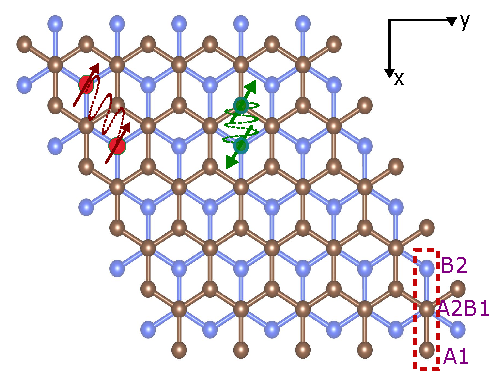
\includegraphics[width=\linewidth]{figures/BLG_regv3.pdf}

\vspace{0.5cm}
{\tiny\color{citegray} RKKY in bilayer graphene:\\
Jiang et al., J. Phys.: Condens. Matter 24, 206003 (2012)\\
Parhizgar, Sherafati, Asgari, Satpathy, PRB 87, 165429 (2013)\\
Klier, Shallcross, Pankratov, PRB 90, 245118 (2014)\par}
\end{column}
\begin{column}{0.58\textwidth}
\vspace{0.1cm}
4-band tight binding, \colorbox{citron!40}{\mystrut fitted to infrared spectra}
\vspace{0.2cm}

{\footnotesize\setlength{\tabcolsep}{3pt}
\begin{tabular}{@{}c c l@{}}
 parameter & value (eV) & what it does\\ \hline
 $\gamma_0$ & 3.16 & in-plane A--B hopping\\
 $\gamma_1$ & 0.381 & vertical B1--A2 (stacked sites)\\
 \textcolor<2->{orchid}{$\gamma_3$} & \textcolor<2->{orchid}{0.38} & \textcolor<2->{orchid}{skew A1--B2: trigonal warping}\\
 $\gamma_4$ & 0.14 & skew A1--A2, B1--B2: e--h asym.\\
 $\Delta'$ & 0.022 & stacked-site energy: e--h asym.\\
\end{tabular}\par}

{\tiny\color{citegray} Model: McCann, Koshino, Rep. Prog. Phys. 76, 056503 (2013)\\ Experiment: Kuzmenko et al., PRB 80, 165406 (2009)\par}

\vspace{0.15cm}
\onslide<2->{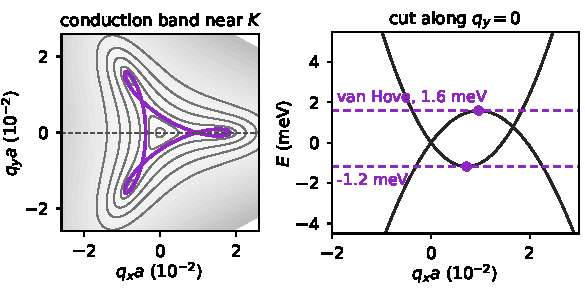
\includegraphics[width=0.97\linewidth]{figures/blg_trigonal_warping.pdf}}
\end{column}
\end{columns}
\end{frame}
% Notes: No twist now; the knob is the impurity position.
% Notes: McCann-Koshino parameters come from infrared spectroscopy on bilayer graphene (Kuzmenko 2009): a realistic host, not a toy.
% Notes: gamma3 gives trigonal warping: near K the conduction band has a central pocket and three leg pockets (left panel).
% Notes: They merge at a saddle point: van Hove singularity at 1.6 meV (and at -1.2 meV in the valence band; gamma4 and Delta' make it asymmetric).
% Notes: Figure made by figures/make_blg_warping.py from the same 4-band model. q is measured from K.
% Notes: This meV structure, three orders of magnitude below gamma0, is why we need a very accurate low-energy (non-)local DoS: next slide.
